\documentclass[a4paper,12pt]{article}
\usepackage{graphicx}
\usepackage{titlesec}
\usepackage[utf8]{inputenc}
\usepackage{xcolor}
\usepackage{fancyhdr}
\usepackage{lipsum}
\usepackage{caption}

\renewcommand{\headrulewidth}{0pt}
\fancyhead[C]{}
\fancyhead[C]{
	
\includegraphics[width=4cm]{metu}
}
\pagestyle{plain}

%opening
\title{Middle East Technical University\\Department of Physics\\\textbf{PHYS307 Applied Modern Physics}}
\author{Oğuzhan ÖZCAN}
\date{}
\clearpage
\thispagestyle{empty}
\providecommand{\groupmember}[1]{\textbf{Group Members:} }
\providecommand{\expdate}[1]{\textbf{Experiment Date:} }
\providecommand{\repdate}[1]{\textbf{Report Submit Date:} }
\providecommand{\expname}[1]{\textbf{Exp. MP-AS Atomic Spectra} }


\usepackage[a4paper,%
left=0.5in,right=0.5in,top=0.5in,bottom=0.8in,%
footskip=.25in]{geometry}
%\topmargin -4.5cm
%\oddsidemargin 0.2cm
%\textwidth 16cm %
%\textheight 21cm%
%\footskip 1.0cm%




\begin{document}
\pagenumbering{gobble}
\maketitle

\thispagestyle{fancy}

%%%%%%%%%%%%%%%%%%%%%%%%%%%%%%%%%%%%%%%%%%%%%%%%%%%%%
\noindent\rule{18.4cm}{0.8pt}
\begin{center}
	\expname{arg1}{}
\end{center}

\expdate{November 6, 2015}{November 20, 2015}\\
\repdate{arg1}{November 27, 2015}\\
\noindent\rule{18.4cm}{0.8pt}\\\\
%%%%%%%%%%%%%%%%%%%%%%%%%%%%%%%%%%%%%%%%%%%%%%%%%%%%%
\begin{table}[h!]

\begin{center}
\begin{tabular}{|c||c|c|c|c|c|c|c|}
	\hline \textbf{Colour}  & $\theta_{R}$ & $\theta_{L}$ &  $\theta$ & $\sin\theta$ & $\lambda$ & Percentage Error & $\Delta\lambda$ \\ 
	\hline \textbf{Violet}  & $164^{\circ}$ & $196^{\circ}26^{\prime}$ & $16.21^{\circ}$ & 0.279 & 4652 \AA & 6.62\% & 590.7 \AA \\ 
	\hline \textbf{Green}  & $160^{\circ}55^{\prime}$ & $197^{\circ}31^{\prime}$ & $18.2^{\circ}$ & 0.312 & 5205 \AA & 8.49\% & 592.9 \AA  \\ 
	\hline \textbf{Yellow} & $159^{\circ}5^{\prime}$ & $201^{\circ}24^{\prime}$ & $20.75^{\circ}$ & 0.354 & 5904 \AA & 0.25\% & 595.9 \AA \\ 
	\hline \textbf{Red} & $158^{\circ}10^{\prime}$ & $202^{\circ}25^{\prime}$ & $22.13^{\circ}$ & 0.376 & 6275 \AA & 1.96\% & 597.5 \AA \\ 
	\hline 
\end{tabular} 
\caption{Spectral lines of Na with the grating (Grating constant d=16666 \AA)}
\end{center}
\end{table}

\begin{table}[h!]
	
	\begin{center}
\begin{tabular}{|c||c|c|c|c|c|c|c|c|c|c|}
	\hline \textbf{Colour} & n & $\theta_{d1}$ & $\theta_{d2}$ & $\sin\theta_{d1}$ & $\sin\theta_{d2}$ & $\lambda_{1}$ & $\lambda_{2}$ &  $\Delta\lambda_{exp}=\lambda_{1}-\lambda_{2}$ & $\Delta\lambda_{theo}$ & $ \Delta\lambda_{p.err}$ \\ 
	\hline \textbf{Red} & 2 & $223.60^{\circ}$ & $223.65^{\circ}$ & .6896 & .6902 & 5746 \AA & 5751 \AA & 5 \AA & 3 \AA  & 66.7\% \\ 
	\hline \textbf{Red} & 3 & $250.28^{\circ}$ & $250.35^{\circ}$ & .9413 & .9417 & 5229 \AA & 5231 \AA & 2 \AA & 2 \AA & 0 \\ 
	\hline \textbf{Yellow} & 2 & $221.61^{\circ}$ & $221.68^{\circ}$ & .6640 & .6649 & 5533 \AA & 5540 \AA & 7 \AA & 3 \AA & 75.0\% \\ 
	\hline \textbf{Yellow} & 3 & $243.25^{\circ}$ & $243.4^{\circ}$ & .8929 & .8941 & 4960 \AA & 4967 \AA & 7 \AA & 3 \AA & 75.0\% \\ 
	\hline \textbf{Green} & 2 & $220.16^{\circ}$ & $220.21^{\circ}$ & .6449 & .6455 & 5373 \AA & 5378 \AA & 5 \AA & 2 \AA & 150\% \\ 
	\hline \textbf{Green} & 3 & $233.8^{\circ}$ & $234.230^{\circ}$ & .8069 & .8113 & 4482 \AA & 4507 \AA & 25 \AA & - & - \\ 
	\hline 
\end{tabular} 
\caption{Fine structure of some spectral lines of Na (Grating constant d=16666 \AA)}
\end{center}
\end{table}
An example calculation for $\Delta\lambda$ where
\begin{equation}
\Delta\lambda=\lambda\sqrt{(\frac{\Delta\theta}{\theta})^{2}+(\frac{\Delta d}{d})^{2}}
\end{equation}
For yellow colour; d=16666 \AA, $\Delta\theta=2^{\circ}$, $\Delta d =500$ \AA, $\theta=20.75^{\circ}$ and $\lambda=5904$ \AA
\newpage
\begin{equation}
\Delta\lambda=5904 \AA \sqrt{(\frac{2^{\circ}}{20.75^{\circ}})^{2}+(\frac{500 \AA }{16666 \AA })^{2}}
\end{equation}
\begin{equation}
\Delta\lambda=5904 \AA \sqrt{9.29\times 10^{-3} + 9.0\times 10^{-4}}
\end{equation}
Therefore
\begin{equation}
\Delta\lambda=595.98 \AA 
\end{equation}
\textit{Remark:} Percentage error is calculated according to following equation
\begin{equation}
\% error= \frac{|Experimental Value - Theoretical Value|}{Theoretical Value} \times 100
\end{equation}
\begin{table}[h!]
	\begin{center}
\begin{tabular}{|c||c|c|c|c|c|c|}
	\hline \textbf{Colour} & n & $\theta_{1}$ & $\theta_{2}$ & $\lambda_{1}$ & $\lambda_{2}$ & $\Delta\lambda$ \\ 
	\hline \textbf{Red} & 2 & 41.45 & 41.48 & 5516 \AA & 5519 \AA & 3 \AA \\ 
	\hline\textbf{ Red} & 3 & 55.96 & 56 & 4603 \AA & 4605 \AA & 2 \AA \\ 
	\hline \textbf{Yellow} & 2 & 40.35 & 40.38 & 5395 \AA & 5398 \AA & 3 \AA \\ 
	\hline \textbf{Yellow} & 3 & 53.81 & 53.86 & 4483 \AA & 4486 \AA & 3 \AA \\ 
	\hline \textbf{Green} & 2 & 39.53 & 39.55 & 5304 \AA & 5306 \AA & 2 \AA \\ 
	\hline 
\end{tabular} 
\caption{Theoretical data for fine structure of Na}
\end{center}
\end{table}
Below table has taken from \textit{Experiments in Modern Physics} [1]. Green colour has not 3rd order spectrum that is why I did not calculate $\Delta\lambda_{theo}$ for green in Table 2. An example calculation for n=2 order wavelength of yellow as follows
\begin{equation}
\lambda=\frac{d \sin \theta}{n}
\end{equation}
\begin{equation}
\lambda=\frac{16666 \AA \times \sin 40.35}{2}
\end{equation}
\begin{equation}
\lambda=5395 \AA
\end{equation}
\textbf{1. What is the most important general statement that you can make from the results of the first part of the experiment? Make a comment on the data you have taken.}\\\\
As we know there are three different spectrum: continuous, absorption and emission. In this part we have seen the emission spectrum of sodium. We can realize  emission spectrum by observing background. If background is dark and if we see bright lines that means we are observing emission spectrum as we did in this experiment. This part shows that Sodium has different coloured lines. Each colour can be visible in different diffraction angles.\\\\
\textbf{2. What causes the specta of different elements to differ?}\\\\
Each element has different that means each element releases photons of different color when its atoms return to their lower energy states. Since each atom has many excited states, different colors of light can be emitted by each element. As we realized in this experiment, group of individual colors emitted by an element is called its spectrum. Since the spectrum of each element is unique, spectra can be used like fingerprints to identify unknown elements.
\newpage
\textbf{3. What is the most important general statement that you can make from the results of the second part of the experiment? Make a comment on the data you have taken.}\\\\
In the second part of the experiment, we measured different orders of Sodium atom. The most important thing in this part is fine structure of sodium. Used energy levels were \textit{n=2} and \textit{n=3}. The
energy difference of these two levels is known as fine structure, and is
due to the spin-orbit coupling, the interaction of the orbital angular momentum
with the spin angular momentum. We have seen same yellow lines in Michelson Interferometer Experiment \textit{(PHYS222 Optics and Waves Laboratory Exp. OW-6)}.\\\\
\textbf{4. If the agreement between the obtained experimental data and the values given in Figure 1 (see Appendix) is fair, explain what could be the source of error in the measured values.}\\\\
Actually our experimental result and theoretical values are very close to each other in the first part of the experiment. However, in the second part of the experiment, percentage error is very high. As we know, grating spectrometer that we used in the experiment is old fashioned. We had to align manually and we had to read degree of spectrometer. Since spectrometer has its own error causes whose stated in lab manual, we have also some errors caused by eyes. We were observing lines with naked eyes and sometimes observing black line was difficult.\\\\
\textbf{5. What is the advantage of using higher orders in diffraction pattern, rather than the first order?}\\\\
Sodium atom has 11 electron therefore electron configuration is $1s^{2}$ $2s^{2}$ $2p^{6}$ $3s^{1}$. In the first order of Sodium, we observe a spectrum which is very familiar with Hydrogen spectrum. However, when we observe 2nd and 3rd order we can see bright doublet sodium spectrum which is known as Sodium D-lines [2] and this line can be observed at 5890 \AA  of the $3S_{1/2}-3P_{3/2}$ transition [3]. Another advantage of using higher orders is that the Sodium doublet is further spit by the application of an external magnetic field which is known as Zeeman Effect.\\\\
\textbf{Discussion and Conclusion}\\\\
In this experiment we studied an important topic in physics and chemistry which is known as spectrum of an atom. This experiment shows us an atom can have different quantum number and these quantum numbers can have different emission spectrums. We conclude this results while doing experiment because we saw very different in the second part. For instance in the second part we did not observe violet colour line. Indeed, this experiments requires further readings it because atomic spectra is a wide topic. If we want to talk about this topic widely, we need to mention Bohr's atom theory, selection rules for related elements, Hydrogen like atoms, Coulomb degeneracy and etc [4]. If we look at the experimental results and theoretical values we can state that the first part of experiment is very succesful it is because we have very low percentage error. However, in the second part of experiment percentage error starts to increasing. Actually I could not realize the cause of these high percentage errors. As I mentioned before I calculated $\Delta\lambda_{theo}$ values in Table 2 according to values are given in Table 3. I am not sure about these values but they seems like that they are correct. By the way, while I was scanning literature, I saw that most of books do not mention \textit{n=3} order for green colour. For instance, Melissinos and Napolitano [1] stated \textit{n=2} and \textit{n=4} quantum numbers for green colour, not for \textit{n=3}. To sum up, in my opinion, experiment is accomplished at least for first part. I wish we would observe other elements' spectrums such as Hyrdogen and Mercury. That would be beneficial for us to understand the difference of spectrums.
\newpage
\textbf{References}\\\\
$[1]$ A. Melissinos, \textit{Experiments in Modern Physics} (Academic
Press Inc., 1966) p.38.\\\\
$[2]$ Irodov, I. (1983). \textit{Problems in Atomic and Nuclear Physics} p.43. Moscow: Mir.\\\\
$[3]$ Haroche, S., Gross, M., \& Silverman, M. P. (1974). \textit{Observation of fine-structure quantum beats following stepwise excitation in sodium D states.} Physical Review Letters, 33(18), 1063.\\\\
$[4]$ Hecht,  E. (2002). Optics (4th ed.)  p.480.  Reading,  Mass.:  Addison-Wesley\\\\\\
\textbf{Appendix}
\begin{figure}[h!]
\centering
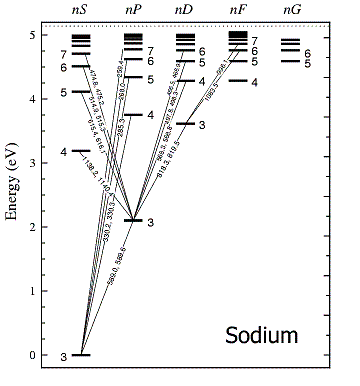
\includegraphics[width=0.7\linewidth, height=0.5\textheight]{Capture}
\caption{Energy level diagram for sodium}
\label{fig:Capture}
\end{figure}













































































































































\end{document}
